\documentclass[11pt,a4paper]{article}
\usepackage[T1]{fontenc}
\usepackage[utf8]{inputenc}
\usepackage[american,spanish,es-noshorthands,es-tabla]{babel}
\usepackage{lmodern}
\usepackage[margin=2.2cm]{geometry}
\usepackage{graphicx}
\usepackage{booktabs}
\usepackage{tabularx}
\usepackage{float}
\usepackage[autostyle=false,style=english]{csquotes}
\usepackage[backend=biber,style=ieee,sorting=none,autolang=other,maxcitenames=6,mincitenames=1,maxbibnames=6,minbibnames=1]{biblatex}
\addbibresource{referencias.bib}
\renewcommand*{\mkpagegrouped}[1]{#1}
\DeclareFieldFormat{eid}{Art. no.~#1}
\usepackage[hidelinks]{hyperref}

\begin{document}

% ------------------------------------------------------------ CARÁTULA
\begin{titlepage}
  \centering
  
\includegraphics[width=3.2cm]{logo uteq.png}\par\vspace{0.6cm}
  {\large\bfseries UNIVERSIDAD TÉCNICA ESTATAL DE QUEVEDO\par}
  \vspace{0.2cm}
  {\bfseries Facultad de Ciencias de la Computación\par}
  {\bfseries Carrera de Software\par}
  \vspace{1.2cm}
  {\bfseries Asignatura:} Aplicaciones Distribuidas\par
  \vspace{0.3cm}
  {\bfseries Actividad:} FORM-AC-01, Análisis de caso: fallo real en un sistema distribuido\par
  \vspace{0.6cm}
  {\Large\bfseries Caída de X (antes Twitter) del 10 de marzo de 2025\par}
  \vspace{1.2cm}
  {\bfseries Docente:} Ing. Gleiston Cicerón Guerrero Ulloa\par
  \vspace{0.3cm}
  {\bfseries Equipo MPZ:}\par
  Muñoz Vera Melanie Michelle\par
  Pozo Castillo Steven Fernando\par
  Zambrano Yong Angel Daniel\par
  \vspace{0.3cm}
  {\bfseries Curso:} Séptimo nivel, paralelo B\par
  \vspace{0.3cm}
  {\bfseries Repositorio:}\par
  {\small\url{https://github.com/Melanir/isr701-form-ac-01}\par}
  \vfill
  Quevedo, Los Ríos, Ecuador\par
  15 de noviembre de 2026\par
\end{titlepage}
\setcounter{page}{1}

% ------------------------------------------------------------ 1 (Melanie)
\section{Descripción del incidente}
El lunes 10 de marzo de 2025 la red social X, antes Twitter, tuvo varias caídas durante el día en Estados Unidos, Reino Unido y otros países. Los usuarios no podían cargar el feed ni publicar, y el servicio volvía por momentos para caerse otra vez \cite{ap2025musk,maruf2025x}. X no publicó un informe post-mortem; lo único oficial son las declaraciones de su dueño, Elon Musk, quien habló de un \enquote{ciberataque masivo} hecho con muchos recursos \cite{ap2025musk}. La Tabla~\ref{tab:linea} resume la línea de tiempo. Las horas están en hora del Este de EE.\,UU. (EDT, UTC$-$4), porque el horario de verano había empezado el día anterior.

\begin{table}[H]
  \centering
  \caption{Línea de tiempo del 10 de marzo de 2025.}
  \label{tab:linea}
  \small
  \begin{tabularx}{\textwidth}{llX}
    \toprule
    EDT & UTC & Evento \\
    \midrule
    5:45  & 9:45  & Empiezan las oleadas de denegación de servicio, según una fuente de la industria de infraestructura \cite{reuters2025musk}. \\
    6:00  & 10:00 & Primer pico en Downdetector, con hasta 20\,538 reportes \cite{maruf2025x}. \\
    10:00 & 14:00 & Segundo pico, con más de 40\,000 reportes \cite{ap2025musk}. \\
    12:00 & 16:00 & Empieza la caída más larga del día, de al menos una hora \cite{ap2025musk}. \\
    14:00 & 18:00 & Los reportes empiezan a bajar y siguen cayendo en la tarde \cite{maruf2025x}. \\
    16:00 & 20:00 & En una entrevista con Fox Business, Musk dice que el ataque usó IP de la zona de Ucrania \cite{maruf2025x}. \\
    \bottomrule
  \end{tabularx}
\end{table}

% ------------------------------------------------------------ 2 (Angel)
\section{Causas raíz}
X no publicó un informe post-mortem del incidente, así que las causas se reconstruyen con el análisis de tráfico de Bitsight \cite{bitsight2025ddos} y el reporte de actividad DDoS de NETSCOUT \cite{netscout2025march}. La Figura~\ref{fig:ishikawa} las agrupa en cuatro categorías y separa el detonante (D) de las causas de fondo (F).

\begin{figure}[H]
  \centering
  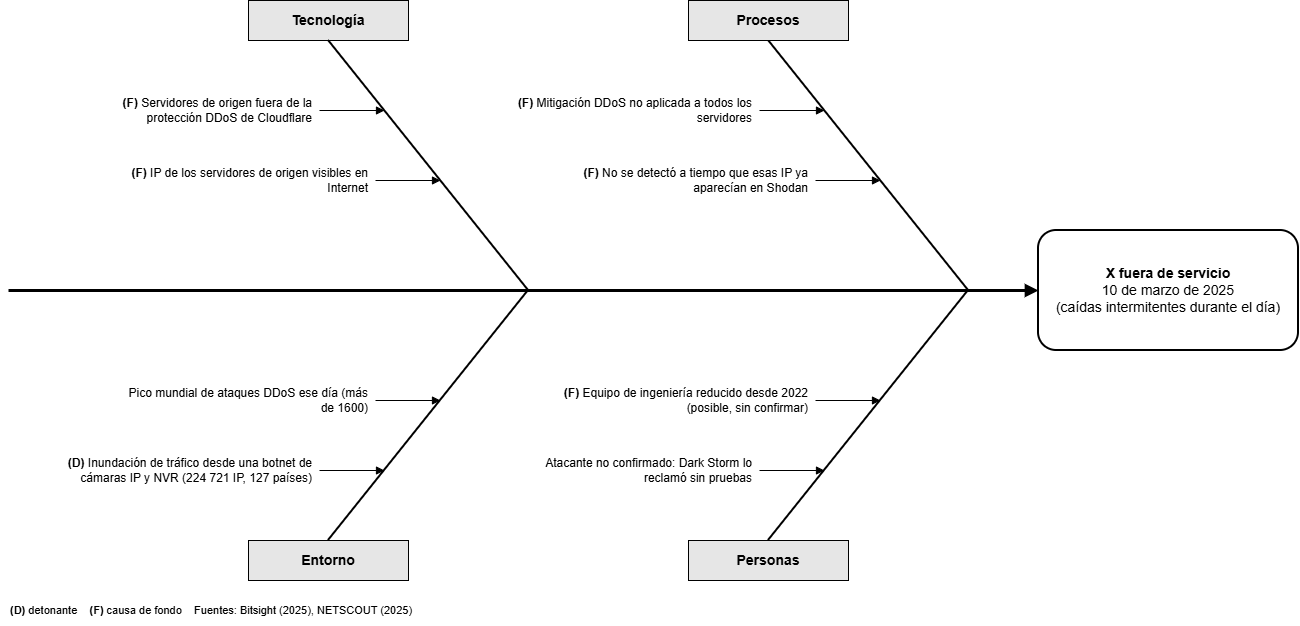
\includegraphics[width=0.8\textwidth]{Ishikawa_X_2025.png}
  \caption{Diagrama de Ishikawa de la caída de X del 10 de marzo de 2025 (elaboración propia en draw.io).}
  \label{fig:ishikawa}
\end{figure}

El detonante fue una inundación de tráfico desde una botnet. En la muestra de Bitsight de ese día hubo 2\,983\,876\,847 paquetes enviados desde 224\,721 direcciones IP de 127 países, y la mayor parte venía de cámaras IP y grabadores de video (NVR) infectados \cite{bitsight2025ddos}. Ese mismo día NETSCOUT registró el pico del mes, con más de 1600 ataques DDoS en el mundo \cite{netscout2025march}.

La causa de fondo es que algunos servidores de origen de X no estaban detrás de la protección DDoS de Cloudflare y sus IP eran visibles desde Internet; incluso aparecían en Shodan \cite{bitsight2025ddos}. Por eso el tráfico pudo ir directo a esos servidores sin pasar por el filtro. La reducción del equipo de ingeniería desde 2022 la dejamos como posible causa, porque ninguna de las fuentes la confirma. La autoría tampoco está clara: el grupo Dark Storm reclamó el ataque, pero Bitsight encontró que sus ataques anteriores usaban otra infraestructura, como routers MikroTik, proxies abiertos y Tor \cite{bitsight2025ddos}.

% ------------------------------------------------------------ 3 (Melanie)
\section{Impacto cuantificado}
En Estados Unidos se superaron los 40\,000 reportes de falla en Downdetector en el pico de las 10:00 EDT \cite{ap2025musk}, y en Reino Unido hubo más de 10\,800 \cite{reuters2025musk}. El 56\,\% de los reportes fue sobre la aplicación y el 33\,\% sobre el sitio web \cite{ap2025musk}. Contando desde el primer pico hasta que los reportes empezaron a bajar, el servicio estuvo inestable unas ocho horas \cite{maruf2025x}. Estas cifras son reportes que envían los propios usuarios, así que no muestran el total de afectados \cite{maruf2025x}. X no publicó pérdidas económicas ni datos de incumplimiento de SLA, por lo que esa parte del impacto no se puede cuantificar con las fuentes disponibles.

% ------------------------------------------------------------ 4 (Angel)
\section{Relación con la Unidad 1}
\textbf{Transparencia rota.} Se rompió la transparencia de fallos, porque los usuarios vieron la caída en lugar de que el sistema la ocultara. También falló la de ubicación: una red de distribución de contenido debería esconder dónde están los servidores reales, y el ataque funcionó precisamente porque esas direcciones estaban expuestas.

\textbf{Teorema CAP.} La propiedad que se perdió fue la disponibilidad, porque los servidores saturados no podían responder a peticiones legítimas. Sin embargo, el CAP habla de lo que se sacrifica cuando hay una partición de red, y ninguna fuente muestra que la red interna de X se haya dividido. Para afirmarlo haría falta saber si los centros de datos de X perdieron comunicación entre sí durante el ataque, y X no publicó ese dato.

\textbf{Mecanismo de tolerancia a fallos que no funcionó.} El mecanismo que quedó corto fue el filtrado de tráfico en el borde, es decir, la mitigación DDoS de la CDN. Estaba pensada para absorber el tráfico malicioso antes de que llegue a los servidores, pero no cubría a todos los servidores de origen, así que una parte del sistema quedó sin protección.

% ------------------------------------------------------------ 5 (Steven)
\section{Mitigación aplicada por la empresa}
X no publicó un informe post-mortem ni una descripción técnica de las acciones ejecutadas para recuperar el servicio. Una fuente de inteligencia de seguridad informó que la empresa activó la protección DDoS de Cloudflare, incluida la presentación de desafíos a conexiones sospechosas \cite{fieldeffect2025x}. Esta medida es coherente con el problema observado por Bitsight: algunos servidores de origen estaban expuestos a Internet y podían recibir tráfico sin pasar por la protección de Cloudflare \cite{bitsight2025ddos}. Sin embargo, al no existir una confirmación técnica de X, no es posible asegurar qué servidores fueron incorporados a la protección ni en qué momento se realizó el cambio.

Como segunda fuente complementaria, Cisco ThousandEyes observó que la disponibilidad se recuperó de forma intermitente durante el día y que no hubo anuncios ni cambios de rutas BGP visibles asociados al dominio de X. Por ello, su análisis sugiere que la mitigación ocurrió dentro de la propia red de X, aunque no permite identificar si se aplicó filtrado, limitación de tráfico u otro mecanismo específico \cite{hicks2025disruptions}. Tampoco hay evidencia pública de cambios permanentes posteriores, como una auditoría de servidores de origen, nuevas reglas de filtrado o modificaciones de arquitectura. En consecuencia, la recuperación del servicio sí es observable, pero el procedimiento exacto y las medidas adoptadas después del incidente permanecen sin confirmar.

% ------------------------------------------------------------ 6 (Steven)
\section{Lecciones aprendidas para el proyecto}
La Tabla~\ref{tab:lecciones} recoge tres riesgos de nuestro proyecto fin de curso que podrían terminar en una caída parecida, con la medida que incorporaremos en TA-PFC-E1.

\begin{table}[H]
  \centering
  \caption{Riesgos del PFC y medidas preventivas.}
  \label{tab:lecciones}
  \small
  \begin{tabularx}{\textwidth}{XX}
    \toprule
    Riesgo & Medida preventiva en TA-PFC-E1 \\
    \midrule
    El servidor de la API queda con su IP y puerto abiertos a Internet, como los servidores de origen de X. & Publicar solo el proxy inverso y aceptar en la API únicamente el tráfico que viene de él. \\
    Un solo cliente puede mandar peticiones sin límite y saturar el servicio. & Limitar las peticiones por IP y por usuario en el proxy o en el API gateway. \\
    Nadie se entera de la caída hasta que los usuarios reclaman, y no hay registro de lo que pasó. & Agregar chequeos de salud, alertas y un registro de incidentes con hora, causa y solución. \\
    \bottomrule
  \end{tabularx}
\end{table}

% ------------------------------------------------------------ DECLARACIÓN DE IA
\section*{Declaración de uso de inteligencia artificial}
El equipo usó Claude (Anthropic), modelo Claude Opus 5.5, para buscar las fuentes, armar el diagrama de Ishikawa en draw.io y redactar el borrador de todas las secciones. Cada integrante revisó la sección a su cargo, comparó cada cifra con la fuente citada y abrió cada URL para comprobar título, autor y fecha.

% ------------------------------------------------------------ REFERENCIAS
\printbibliography[title={Referencias}]

% ------------------------------------------------------------ VERSIÓN FINAL
\section*{Observaciones recibidas y cambios realizados}
Al cierre de esta versión el análisis todavía no se ha expuesto en clase, por lo que el equipo no ha recibido evaluaciones de pares ni observaciones del docente. Cuando se presente, se agregará aquí una tabla con cada observación, quién la hizo y el cambio realizado o la razón para no aplicarlo.

\end{document}
